% Template for ICIP-2019 paper; to be used with:
%          spconf.sty  - ICASSP/ICIP LaTeX style file, and
%          IEEEbib.bst - IEEE bibliography style file.
% --------------------------------------------------------------------------
\documentclass{article}
\usepackage{spconf,amsmath,graphicx}
\usepackage[backend=biber, style=ieee]{biblatex}
\usepackage{float}
\addbibresource{reportRefs.bib}

% Example definitions.
% --------------------
\def\x{{\mathbf x}}
\def\L{{\cal L}}

% Title.
% ------
\title{House Price And Affordability In Regions Of Englanf And Wales}
%
% Single address.
% ---------------
% \name{Author(s) Name(s)\thanks{Thanks to XYZ agency for funding.}}

\name{Junsong Yang}
\address{4274056 \\
psyjy3@nottingham.ac.uk}

\begin{document}
%\ninept
%
\maketitle
%

\section{Introduction}
House price has changes dramatically over the past few years. Such changes are drawing 
attentions as they are leading to housing affordability issues. For example, house price 
in London increased drastically these years, as a result, house price is becoming unaffordable
to most of the residents. Analysis of how the house price changed and 
to what extend the affordability is affected by that changes is provided.

This paper is intend to explore this issue based data about house prices and affordability measurements. 
In general, there are four sections, Initial Question, Data Processing, Information Visualisation and Evaluation.
In Initial Questiions section, issuses related to house prices will be discussed therefore research questions 
will be proposed. As for Data Processing part, information about dataset used in this paper will be briefly 
introduced and how it was processed and data cleaning and transformation process will be explained. 
Visualisation strategies will be discussed in Information Visualisation section alongside visual encoding. 
As for the Evaluation part, evaluation of visualisation will be provided with the general reflection of development process.

\section{Initial Questiions}
As mentioned above, the increase of house price lead affordability concerns. A better understanding of 
the house market, and affordability of the locals are necessary to study this issue. For instance, 
how the house price changed and to what extend that change has influenced affordability. Hence 
the research questions are proposed as follow.

\begin{enumerate}
  \item How the mean house price across the regions changed 
  from 2000 onward and Which region has cheapest house.
  \item How the ratio of house price to workplace-based earnings
  changed from 2000 onward and which region has the most affordable
  houses.
  \item How the house price and affordability was affected by the economy crisis in 2008.
\end{enumerate}

% structures of visualisation part (two graphs at least)
% 1 describe graphs 150 -200
% 2 visualisation strategies 150 - 200
% 3 how those graphs anwsered the question 150 -200
% 4 (optional) further question emerged ? 100 -200



\section{Data Processing}

The dataset, obtained from office for national statistics, contains annual data from 1997 to 2018 about 
the median house price across regions of England and Wales, the median gross annual 
earnings based on working place associated with different regions and the ratio of 
median house price to median gross annual earnings.\cite{henretty_2019} \cite{henretty_data_2019}
In each part, only annual data is provided. 

The data is grouped by regions, counties and local authorities. Data of median house price, median 
affordability ratio and lower quartile house price is provided for each group. The affordability ratio 
refers to the ratio of house price to annual gross earnings. In this case the Affordability ratio was 
calculated as the ratio of median house price to annual gross workplace-based earnings. 
(work-based earnings refers the earnings based on where a person work and does not necessarily reveal 
the earnings of the local residents.)

Data cleaning and filtering process is essential for the project as the dataset has quite a few garbage data. 
As those initial questions suggest, data from 2000 to 2018 will be preserved and analysed, therefore, data 
out of this rage will be purged. As the data provided is completed so the missing data problem does not need 
to deal with. Since the data is also consistant, the entity resolution will not be a problem. 

Type conversion is an issue spacifically related to the R programming language. The original data came in 
xls form with the correct type for each category of data. But when loading those data into R, the default 
data type was character. This issue may cause severe problem whrm performing numeric analysis and visualisation. 
Therefore, data of house price, affordability ratio and data indicating time need to be converted into numeric type. 

As the the annual data is presented seperately in different columns, transformation is needed for further 
data analysis. The original data was put seperately in columns by each year, which would be diffcult to 
analyse changes based on timeline. Hence, the data was trnasformed into three-column form. Name of region, 
year, and the actual values of price (or earnings, or ratios) were in three individual column.

\section{Information Visualisation}
In this section, all three initial question proposed earlier will be discussed with visualisation. 
For each question, visualisation stragies and visual encoding will be explained in detail and 
criticial discussions of visualisation design will be included in this section. After the three initial 
questions were explored, exploratory process of proposing new question and visualisation of that question 
will be explored.

\subsection{House Price Visualisation}
As mentioned earlier, the first question is intend to examine how the house price changed from 2000 to 2018 
and to further probe which region has the lowest house price. As data processing operations described above. 
The first graph can be obtained.

\begin{figure}[H]
  \begin{minipage}[b]{1.0\linewidth}
    \centering
    \centerline{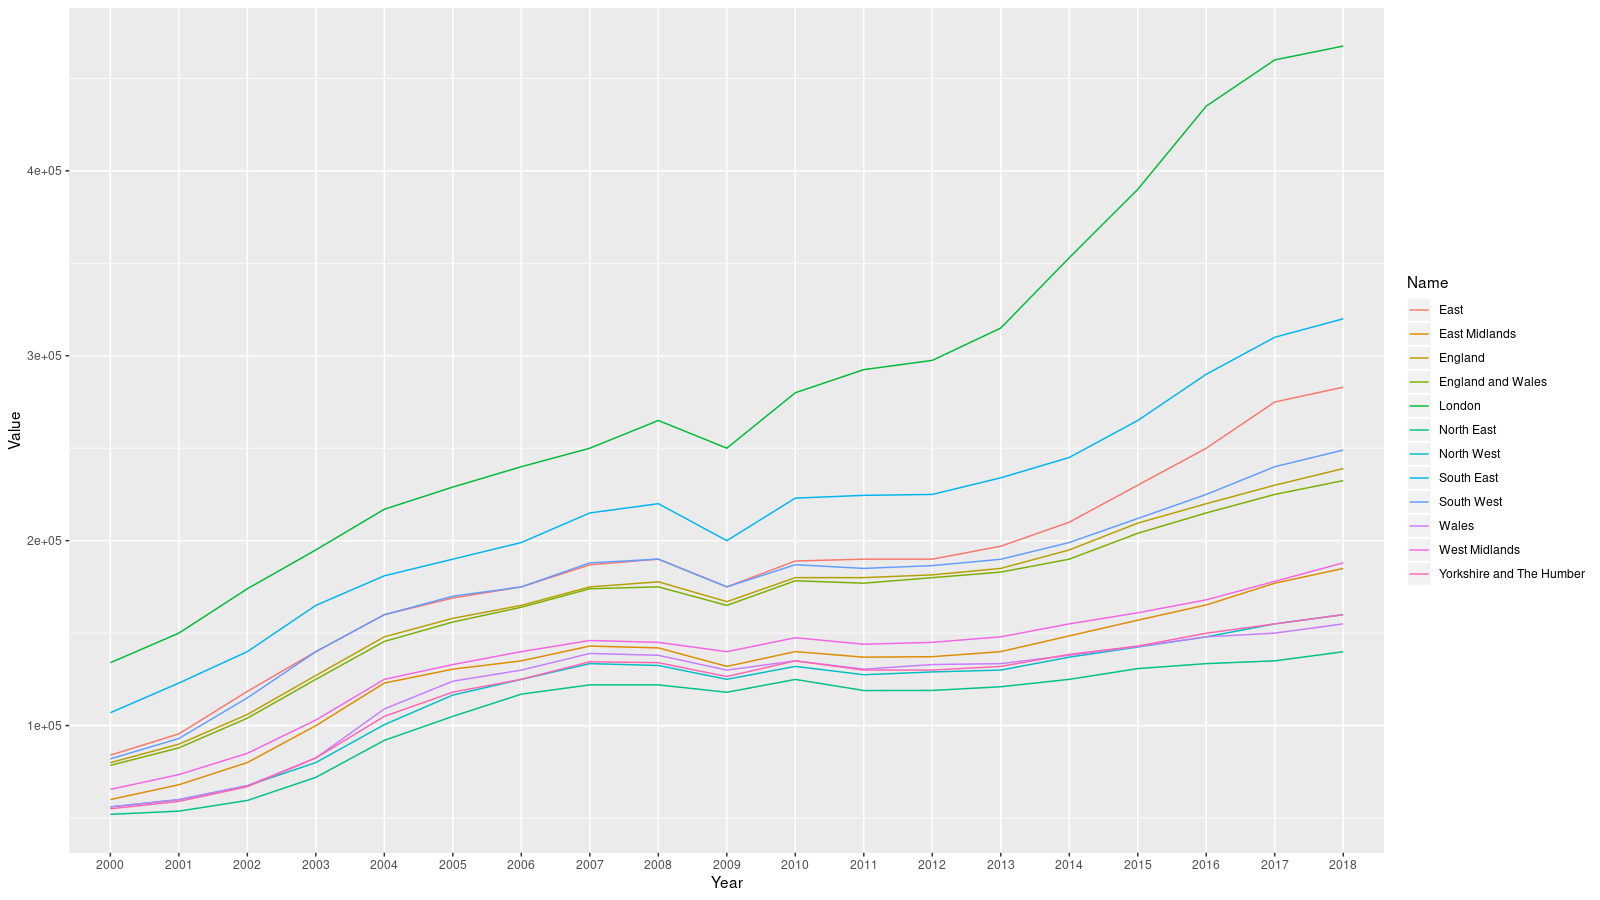
\includegraphics[width=8.5cm]{Q1Geom_line}}
  %  \vspace{2.0cm}
    \centerline{Question 1: Result 1}\medskip
  \end{minipage}
\end{figure}

This line graph illustrate the median house prices in nine regions of England and Wales from 2000 to 2018. 
England and Wales are also treated as regions and also England and Wales combined. Therefore, there 12 lines 
in the graph that represent 12 regions individually. 

The overall tendency of change for all regions is quite similar. Although flucuated for a few years around 2009, 
the median house price in 12 regions was all increased from 2000 to 2018. Staring from 2000, median house 
price in most region rose steadily until 2014. From 2004 to 2008, for all the regions, the increase of 
median house price was slowing down comparing to the increase from 2000 to 2004. For the first time from 2000, 
median house price in all regions suddenly dropped to the level of two years before. Then in 2009, the median 
house price in all regions bounced back to the highest level from 2000. From 2010 onward, the median house 
price was almost fixed for 3 years. Starting from 2013, the median hose price started increasing steadily for 
most regions but London. Median house price in London experienced a sharp increase from 2013 to 2017, 
as the result, the median house price increased by 1/3 compare to the data in 2013. From 2017 onward, 
the increase was slowing down again.

This line graph as an example is expressive and efficient when representing time-series data or the changing 
of quantitative during a continuous period of time. But sometimes, it is not appropriate for conducting 
comparison. Therefore, the second graph was ontained using the same median house price data.

\begin{figure}[H]
  \begin{minipage}[b]{1.0\linewidth}
    \centering
    \centerline{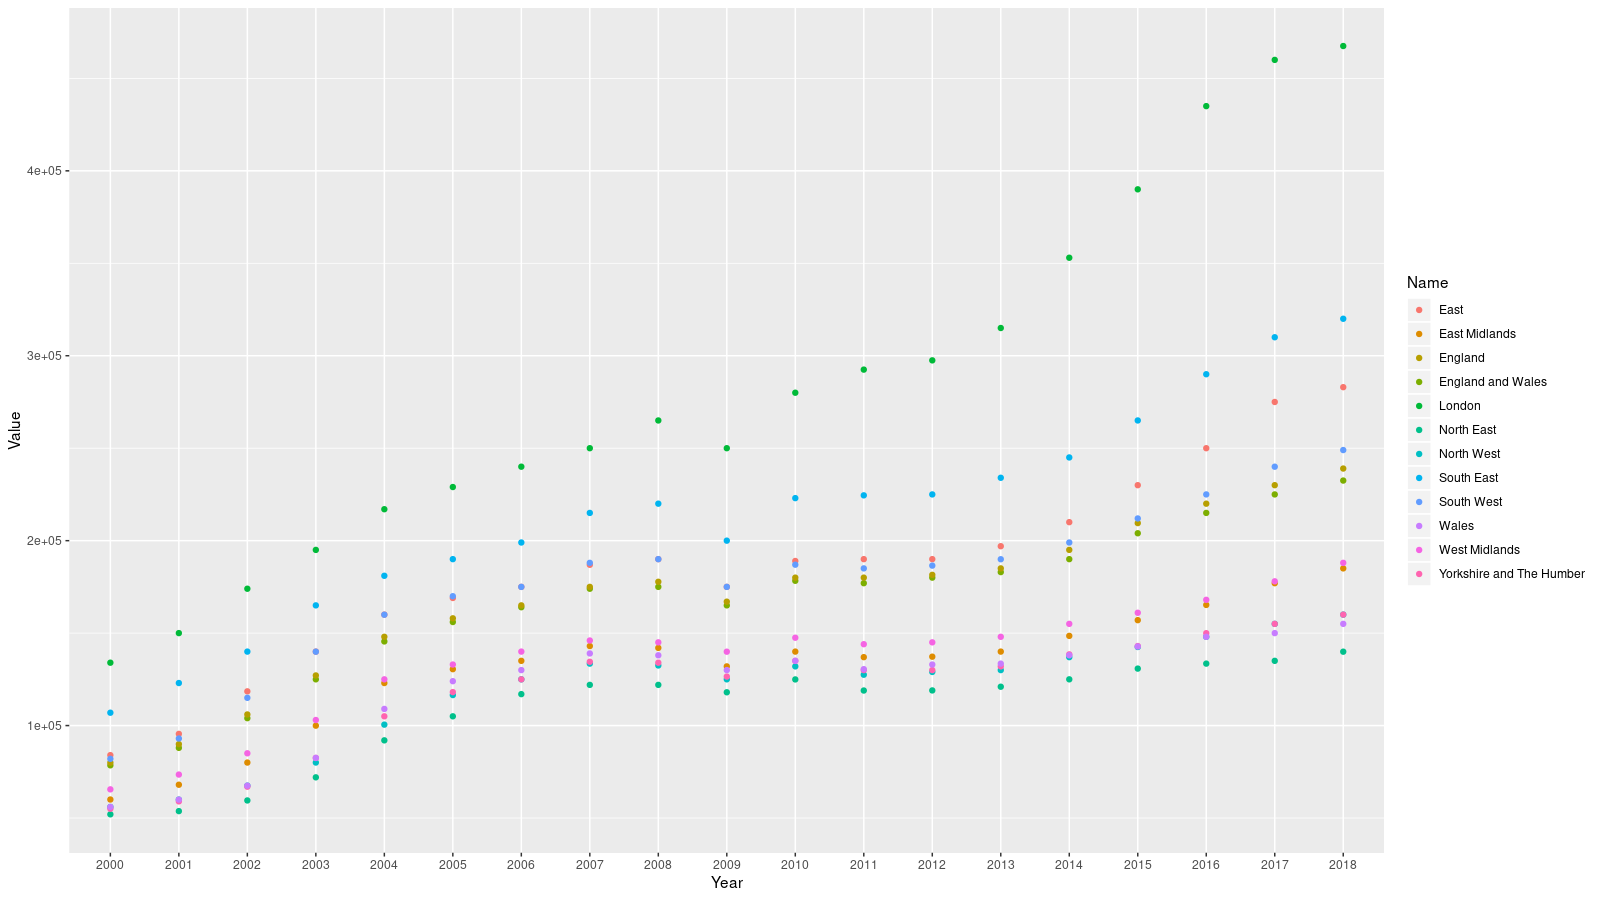
\includegraphics[width=8.5cm]{Q1Geom_point}}
  %  \vspace{2.0cm}
    \centerline{Question 1: Result 2}\medskip
  \end{minipage}
\end{figure}

This dot plot shows the same information as the line graph before but using a different representation. 
By using dot to exhibit the median house price for each region, the comparison of price between different 
region is quite obvious comapre to the line graph due to overlap of line can be observed in line graph 
which caused diffculty to do the comparison.

Based on the dot plot, it is self-evident that the north east region has houses with the lowest median price 
from 2000 to 2018 while London has the most expensive houses.

\begin{figure}[H]
  \begin{minipage}[b]{1.0\linewidth}
    \centering
    \centerline{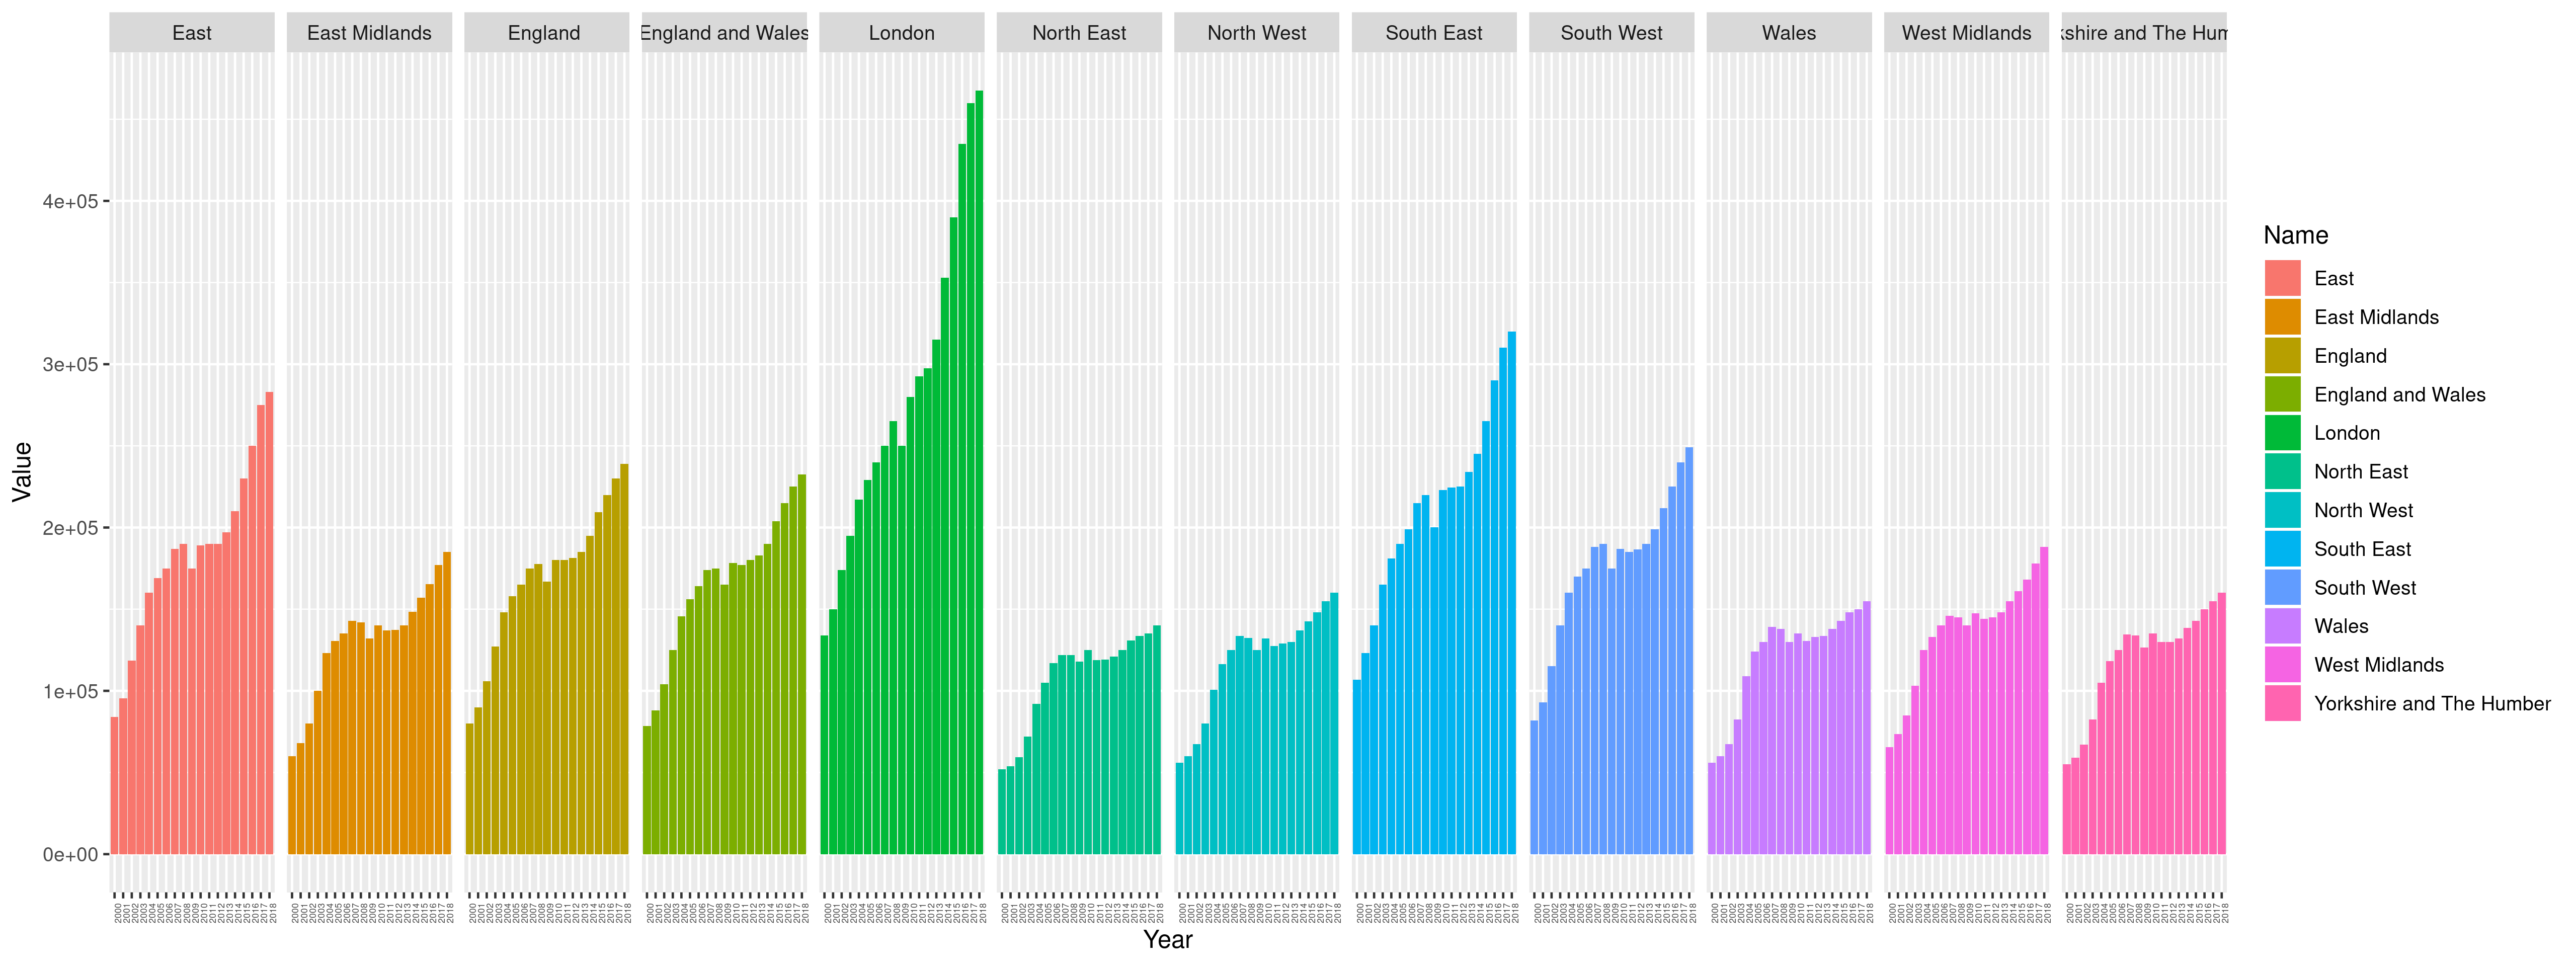
\includegraphics[width=8.5cm]{Q1Geom_gridbar}}
  %  \vspace{2.0cm}
    \centerline{Question 1: Result 3}\medskip
  \end{minipage}
\end{figure}

The last graph for the house price visualisation part is a bar chart which was gained using the same 
median house price data. This bar chart illustrates median house price of 12 regions from 2000 to 2018 
grouped by region. This graph has advantage over the line graph and dot plot when studying the changes of median house price of individual 
regions as it combines the benefit of those two while makes data related to individual region evident.

\subsubsection{Visual Encodings}
Based Bertin's semiology graphics \cite{BertinJacques}, the following characteristics of visual encoding variable 
are taken into considerarion during the visualisation process. 

\begin{itemize}
  \item Selective:
        whether the changes of a variable can make the variable distinctive from the group
  \item Associative:
        whether the changes of a variable can be interperted together as a group
  \item Quantitative: 
        whether the numerical measures can be identified from the changes of a variable
  \item Length:
        how many recognisable changes can be indentified in a variable
\end{itemize}

Combined with the characteristics listed above, there are two principles of choosing visual encodings that 
also need to be enforced. Principle of consistancy refers to the properties of visual variable should match 
the properties of data and the principle of importance ordering refers to encoding the most essential information 
in a most practical manner.

In terms of the line graph for this question, position and hue are selected for the graph. As visual variable, 
position possesses characteristics like selective, associative and quantitative. Moreover, as for 
the length characteristics, theoretically it can be infinite. While hue is selective and associative. As for length, 
the limitation of length when using hue is hardly applied to this dataset. But without hue, the graph is not 
effective nor expressive(See Appendix 1). By combining position and hue together, the line graph was drawed. 

Judging from the desgin criteria, the line graph satififies expressiveness, and partial effectiveness because 
the dot plot is more effective when compare house prices for all regions by year. Therefore, the dot plot was 
obtained to address this issue.

As for the bar chart, position ans hue are combined to achieve expressiveness and effectiveness. It turns out 
that the bar chart is more effective than line graph and dot plot when study the house price of a individual region.




\subsection{Affordability Visualisation}
Stated in the initial question section, the second question is intend to examine how the affordability ratio changed from 2000 to 2018 
and to further probe which region has the most affordable house. Due to the similar nature of the question, 
similar approaches for house price visualisation can be applied here. As data processing operations described above. 
The first graph can be obtained.

\begin{figure}[H]
  \begin{minipage}[b]{1.0\linewidth}
    \centering
    \centerline{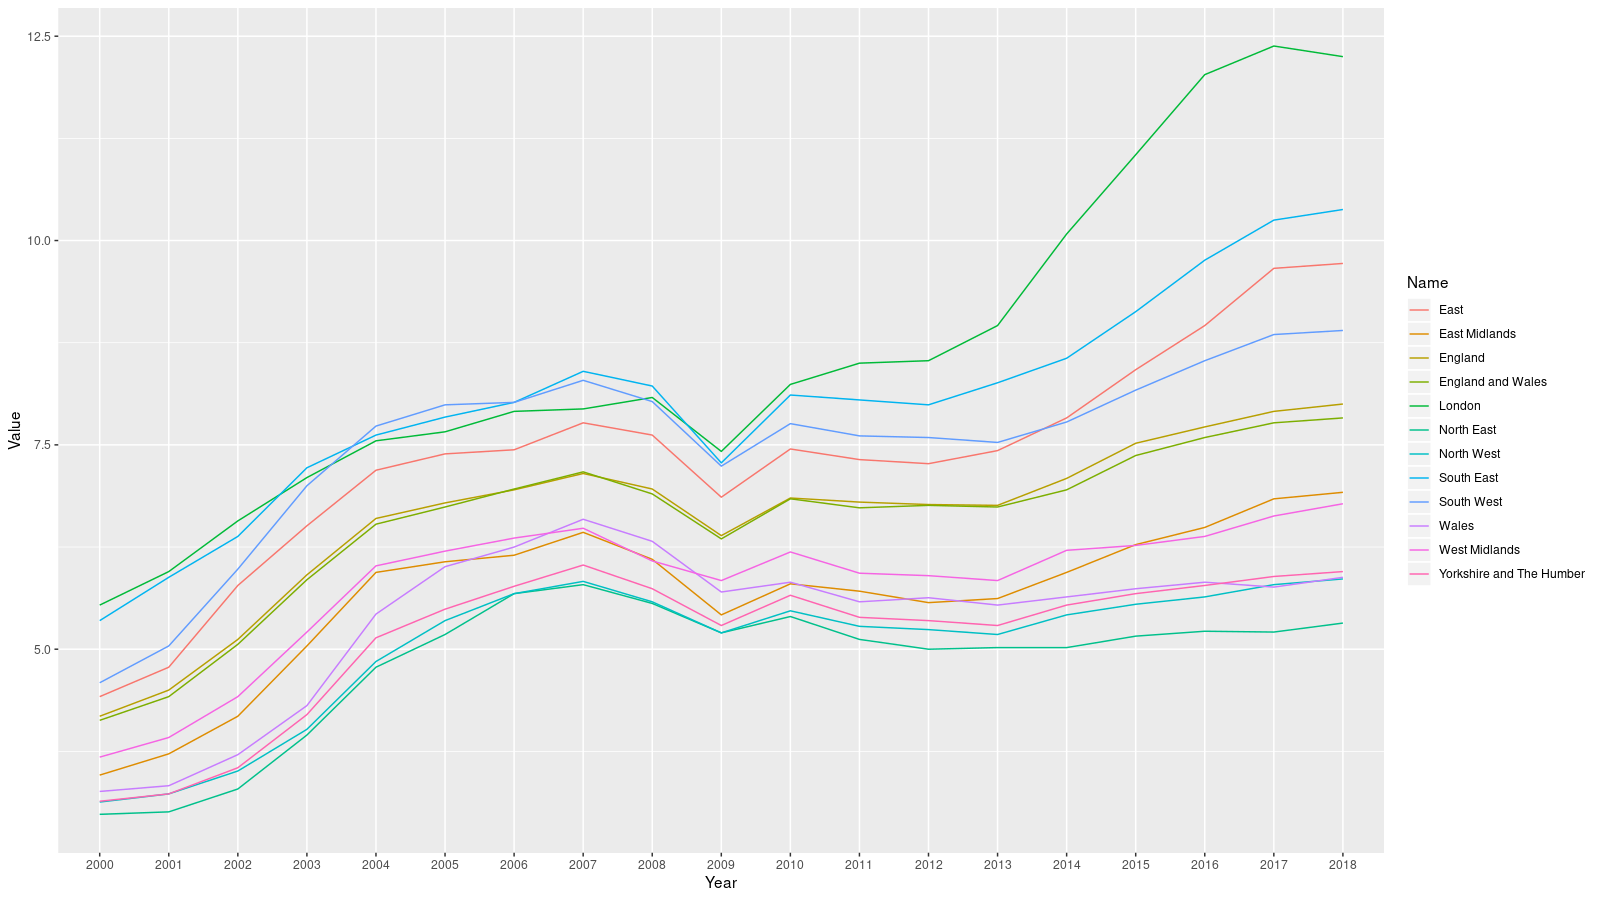
\includegraphics[width=8.5cm]{Q2Geom_line}}
  %  \vspace{2.0cm}
    \centerline{Question 2: Result 1}\medskip
  \end{minipage}
\end{figure}

This line graph illustrate the affordability ratio in nine regions of England and Wales from 2000 to 2018. 
England and Wales are also treated as regions and also England and Wales combined. Therefore, there 12 lines 
in the graph that represent 12 regions individually. As the name suggested, the affordability ratio is the 
ratio of median house price to the median workpace-based earnings. Therefore, the lower the ratio, the more 
affordable the houses are in a region.

The general trend of change for all regions is identical. Although flucuated for a few years around 2009, 
the affordability ratio in 12 regions was all increased from 2000 to 2018. Staring from 2000, affordability ratio 
in most region rose steadily until 2001 and then continued to increase with a faster volocity until 2004. 
From 2004 to 2008, for all the regions, the increase of affordability ratio was almost static for most of 
the regions comparing to the increase from 2000 to 2004. For the first time from 2000, affordability ratio 
in all regions suddenly dropped to the level of four years before. Then in 2010, the affordability ratio in 
all regions bounced back, and from 2010 onward, the affordability ratio was almost fixed for 4 years. Starting from 2013, 
the affordability ratio started increasing steadily for most regions except London. The affordability ratio in London 
started grwoing from 2010 and experienced a sharp upward that last four year and it stil increasing in 2018, 
as the result, the affordability ratio increased by more that 1/3 compare to the data in 2013. Staring from 2013, 
for most region, the affordability ratio started going upwards steadily until 2018.

This line graph as an example is expressive and efficient when representing time-series data or the changing 
of quantitative during a continuous period of time. But sometimes, it is not appropriate for conducting 
comparison. Therefore, the second graph was generated using the same affordability ratio data.

\begin{figure}[H]
  \begin{minipage}[b]{1.0\linewidth}
    \centering
    \centerline{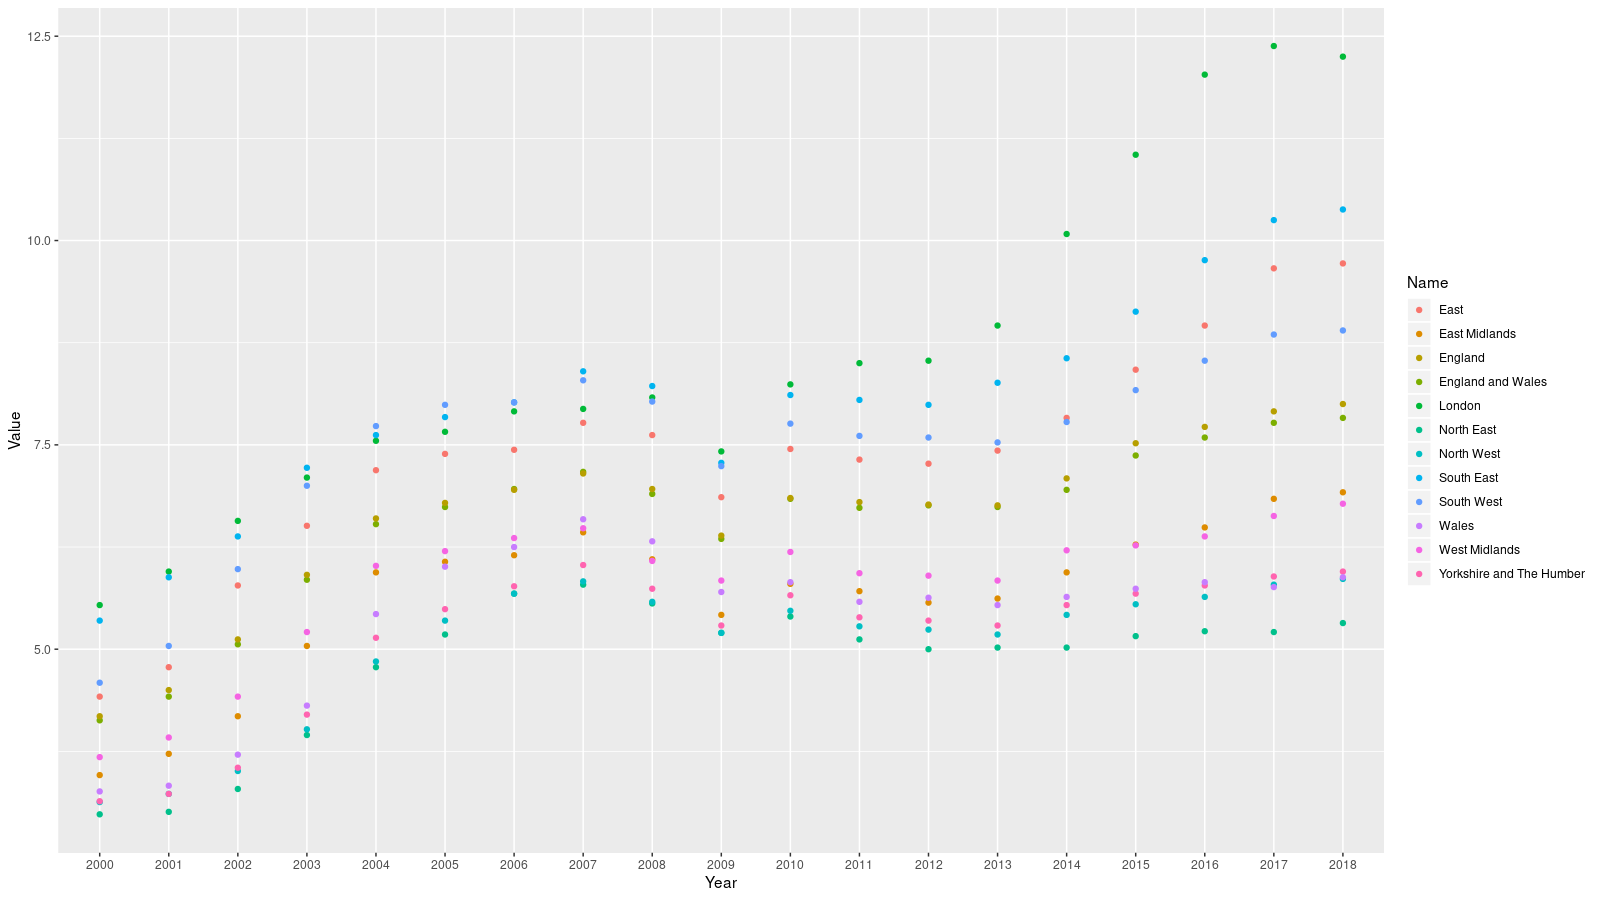
\includegraphics[width=8.5cm]{Q2Geom_point}}
  %  \vspace{2.0cm}
    \centerline{Question 2: Result 2}\medskip
  \end{minipage}
\end{figure}

This dot plot shows the same information as the line graph before but using a different representation. 
By using dot to exhibit the affordability ratio for each region, the comparison of the ratio between different 
region is quite obvious comapre to the line graph due to overlap of line can be observed in line graph 
which caused diffculty to do the comparison.

Based on the dot plot, it is self-evident that the north east region has the most affordable houses from 2000 
to 2018. As the for least affordable houses, the results are interesting compare to the house price. 
As demostrated in house price visualisation part, Houses in London always have the highest price from 2000 to 2018.
But the affordability ratio date suggests that from 2000 to lat 2002, the affordability ratio in London was the lowest 
accross the regions but later on the affordability ratio of south west and south east surpassed the value of London. 
London did not possess the highest value of affordability ratio until late 2018, maintained its statue until 2018.


\begin{figure}[H]
  \begin{minipage}[b]{1.0\linewidth}
    \centering
    \centerline{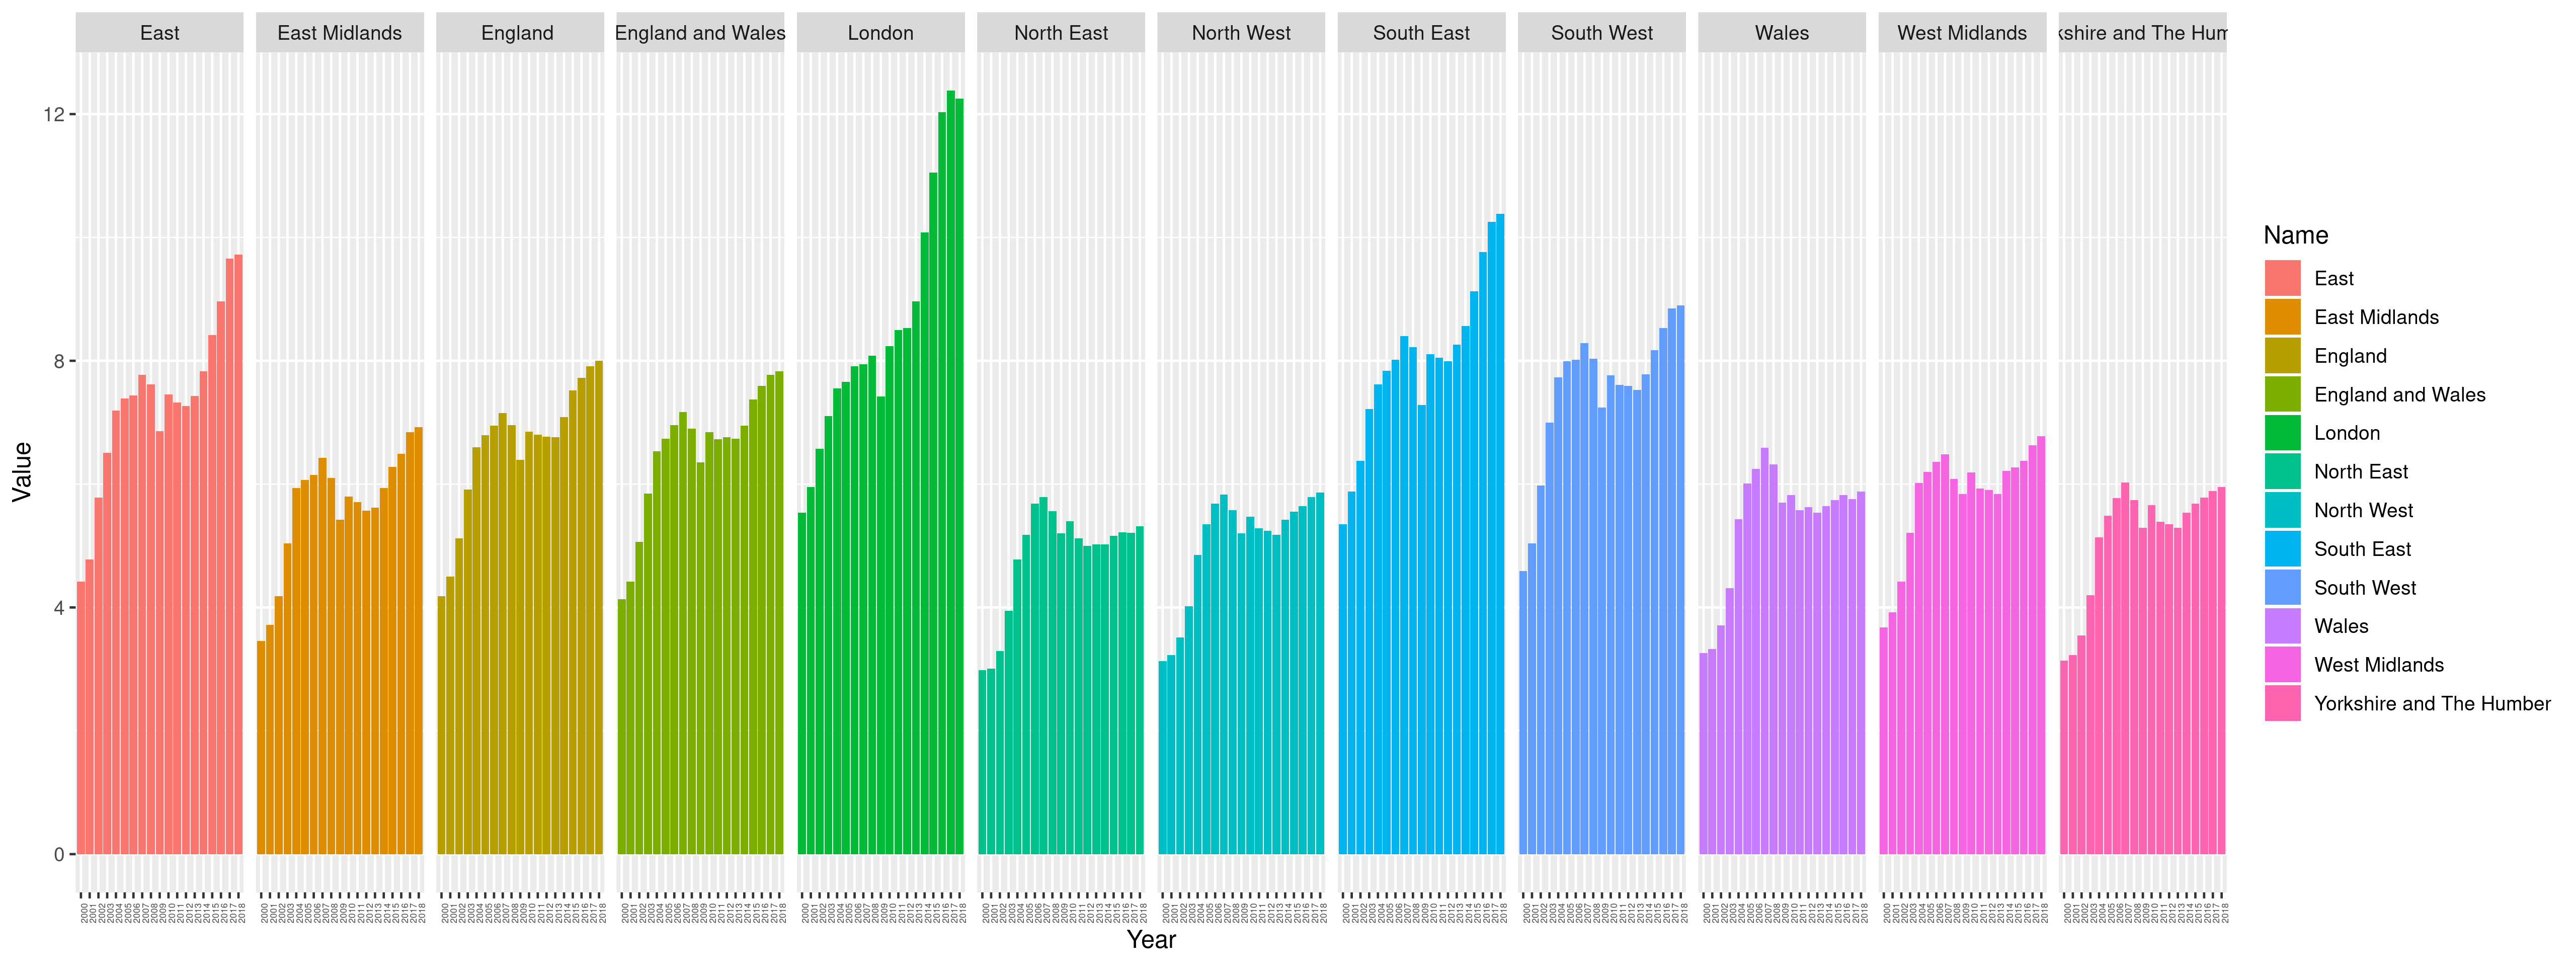
\includegraphics[width=8.5cm]{Q2Geom_gridbar}}
  %  \vspace{2.0cm}
    \centerline{Question 2: Result 3}\medskip
  \end{minipage}
\end{figure}

The last graph for the affordability ratio visualisation part is a bar chart which was gained using the same 
affordability ratio data. This bar chart illustrates affordability ratio of 12 regions from 2000 to 2018 
grouped by region. This graph has advantage over the line graph and dot plot when studying the changes of affordability ratio of individual 
regions as it combines the benefit of those two while makes data related to individual region evident.

\subsubsection{Visual Encodings}
Combined with the characteristics listed above, there are two principles of choosing visual encodings that 
also need to be enforced. Principle of consistancy refers to the properties of visual variable should match 
the properties of data and the principle of importance ordering refers to encoding the most essential information 
in a most practical manner.

In terms of the line graph for this question, position and hue are selected for the graph. As visual variable, 
position possesses characteristics like selective, associative and quantitative. Moreover, as for 
the length characteristics, theoretically it can be infinite. While hue is selective and associative. As for length, 
the limitation of length when using hue is hardly applied to this dataset. But without hue, the graph is not 
effective nor expressive(See Appendix 1). By combining position and hue together, the line graph was drawed. 

Judging from the desgin criteria, the line graph satififies expressiveness, and partial effectiveness because 
the dot plot is more effective when compare house prices for all regions by year. Therefore, the dot plot was 
obtained to address this issue.

As for the bar chart, position ans hue are combined to achieve expressiveness and effectiveness. It turns out 
that the bar chart is more effective than line graph and dot plot when study the house price of a individual region.




\subsection{Impact of Economy Crisis}
The last of initial question is to audit the impact the economy crisis has on house price and affordability
in 12 regions. In this case, the date ned to be processed further. As the economy crisis happened in 2018, 
the comparison of the data in 2008 and 2009 would depict the immdiate impact of the economy crisis. By taking 
in consideration of median house price, annual earnings and affordability ratio, the bar chart can be gained.

\begin{figure}[H]
  \begin{minipage}[b]{1.0\linewidth}
    \centering
    \centerline{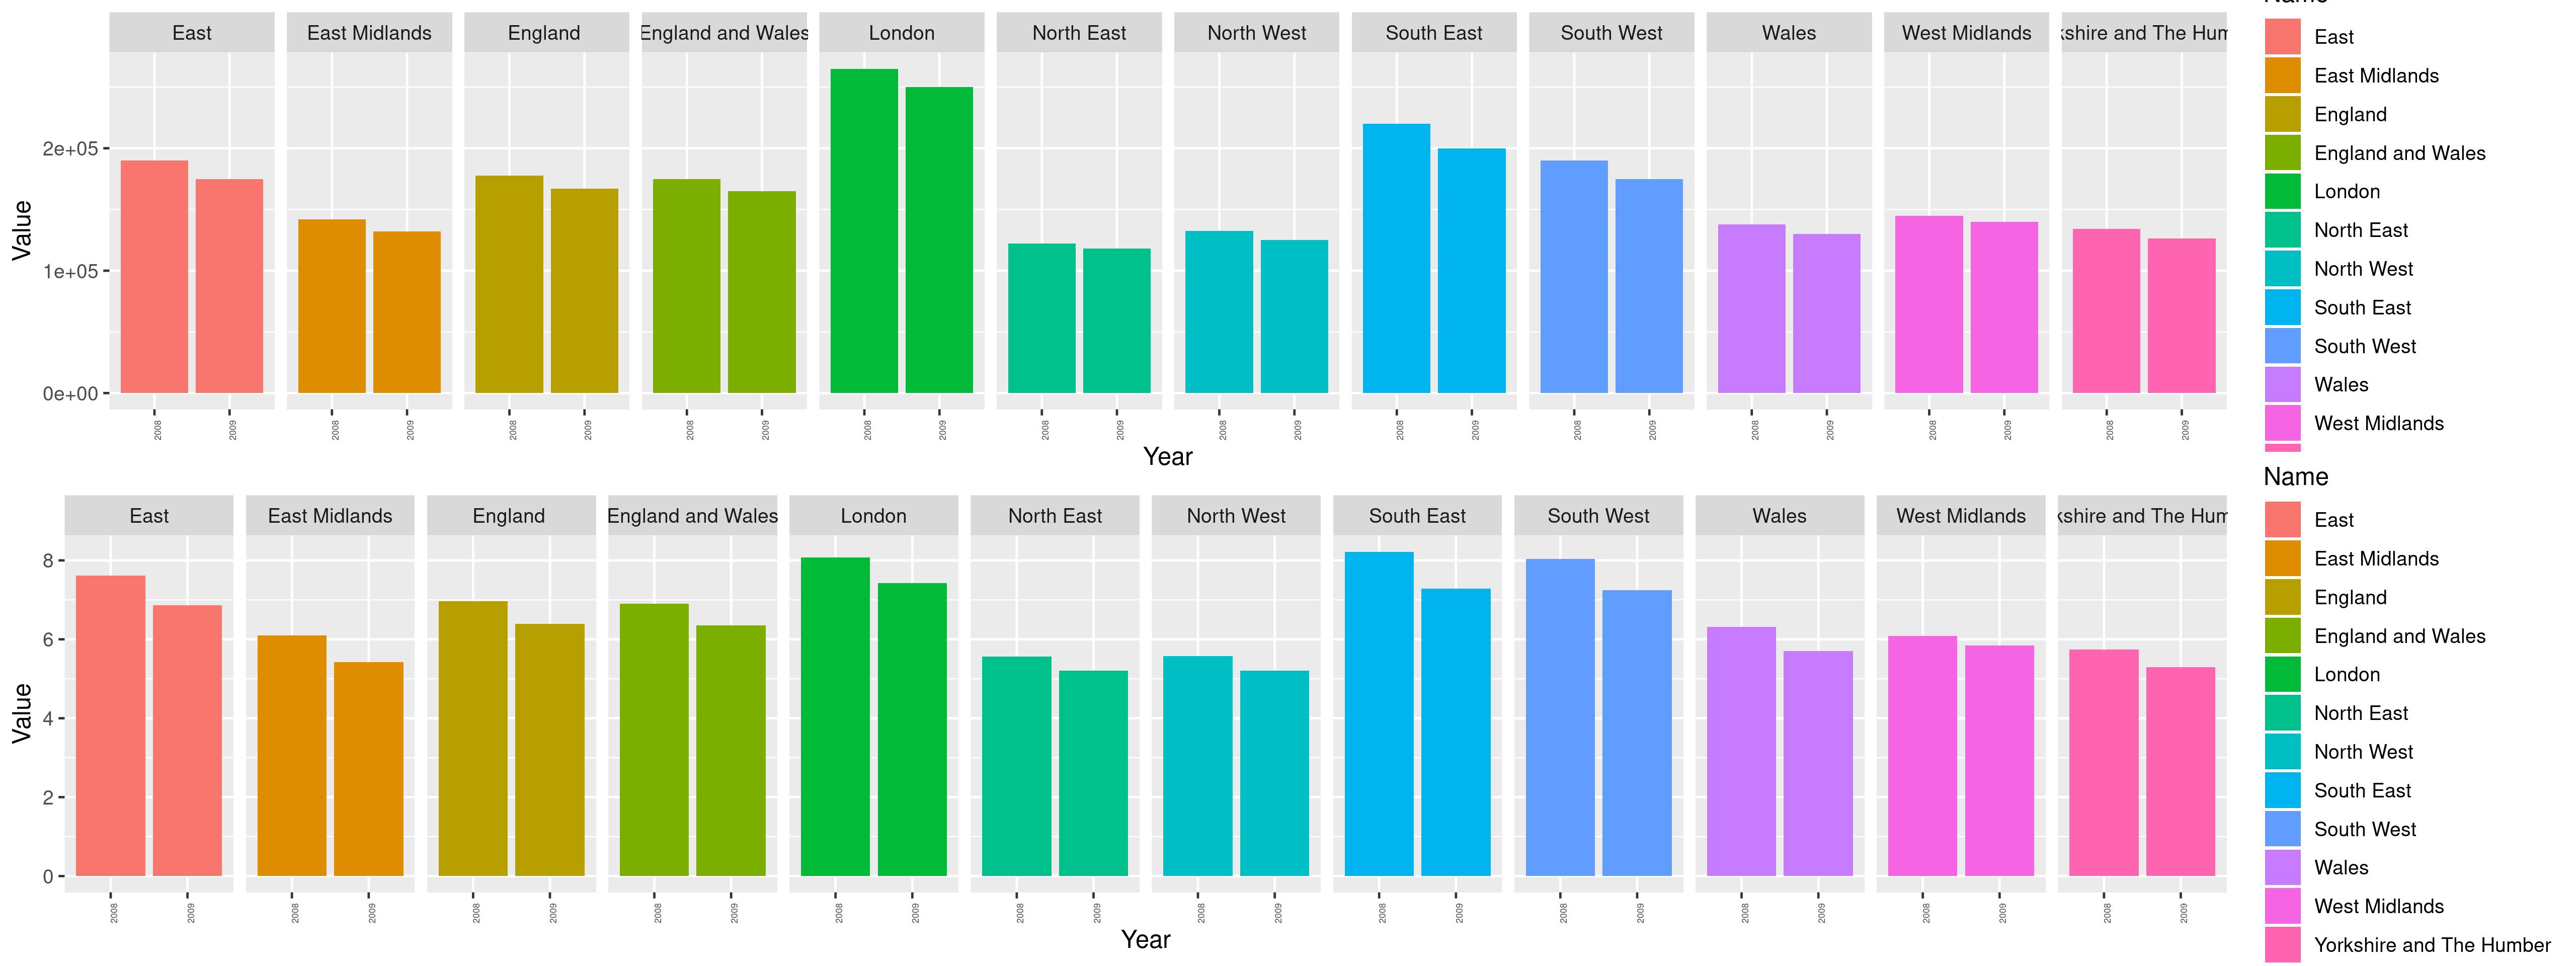
\includegraphics[width=8.5cm]{Q3Geom_gridbar}}
  %  \vspace{2.0cm}
    \centerline{Question 3: Result}\medskip
  \end{minipage}
\end{figure}

This bar chart combines the data of median house price, median annual gross workplace-based earnings and 
affordability ratio from 2008 to 2009. This chart is intend to show the immdiate impact of the economy crisis 
in 2008. As graph shows, the first rwo indicates the annual earning data, the second row represents the median 
house price data and the last row suggests affordability ratio. 

As the graph demostrated, the economy crisis did not seems to have serve impact on annual earnings as the 
annual earnings did not experience any regression in any region. In contract, the impact of the economy crisis 
was obvious, for the house price decreased in all 12 regions. By combining these data, the annual earnings increased 
slightly while the house price decreased, as a result, the affordability ratio decreased. The diminish of 
affordability ratio suggested that the houses in all 12 regions became more affordable as an impact of 
economy crisis. 

\subsubsection{Visual Encodings}

\subsection{Correlation Coefficients of House Price}
As the graphs shown in house price visualisation and affordability ratio visualisation section, the general 
tendency in those regions were quite akin. So that result lead to another question, whether the house prices 
in those regions were related and if they were related how closely they are related to each other.

In search this question, further data transformation is needed. The column in dataset which identify time 
ca be omitted. Furthermore, each region was put in seperate column with all of the data related to the region 
sorted by time. The correlation coefficient is numerical measure the can reveal how diferent entities are 
related to each other. After this transformation, the correlation coefficients can be calculated. Hence, 
the heat map contains correlation coefficients can be obtained.

\begin{figure}[H]
  \begin{minipage}[b]{1.0\linewidth}
    \centering
    \centerline{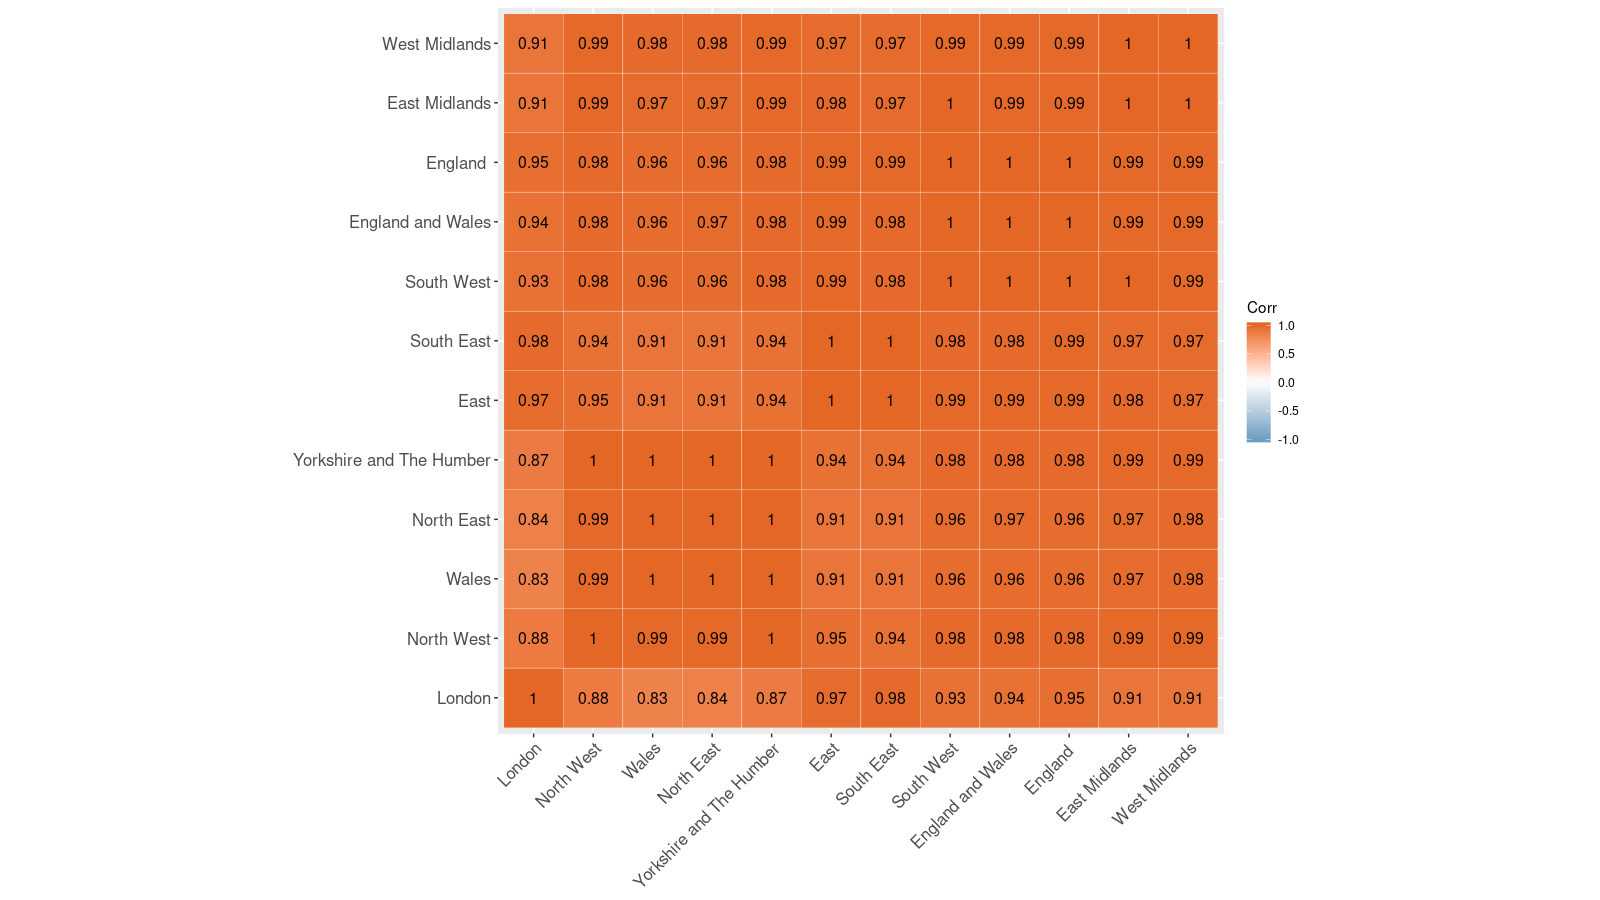
\includegraphics[width=8.5cm]{corHeatMap}}
  %  \vspace{2.0cm}
    \centerline{Correlation Coefficients: Result}\medskip
  \end{minipage}
\end{figure}

As the heat map shows, the correlation coefficients scales from 1 to -1. The close the correlation coefficients 
to 1 the more they are related and vice versa.

As the data suggests, house prices in most region are highlty correlated as most of correlation coefficients 
are above 0.9. Dispite correlation coefficients between some regions are below 0.9, they stil can be 
considered colsely related as they all surpassed 0.8.

\subsubsection{Visual Encodings}




\section{Evaluation}


% To start a new column (but not a new page) and help balance the last-page
% column length use \vfill\pagebreak.
% -------------------------------------------------------------------------
%\vfill
%\pagebreak


\vfill\pagebreak
\printbibliography


\vfill\pagebreak
\vfill\pagebreak

\section*{Appendix}
\subsection{Appendix 1}
\begin{figure}[H]
  \begin{minipage}[b]{1.0\linewidth}
    \centering
    \centerline{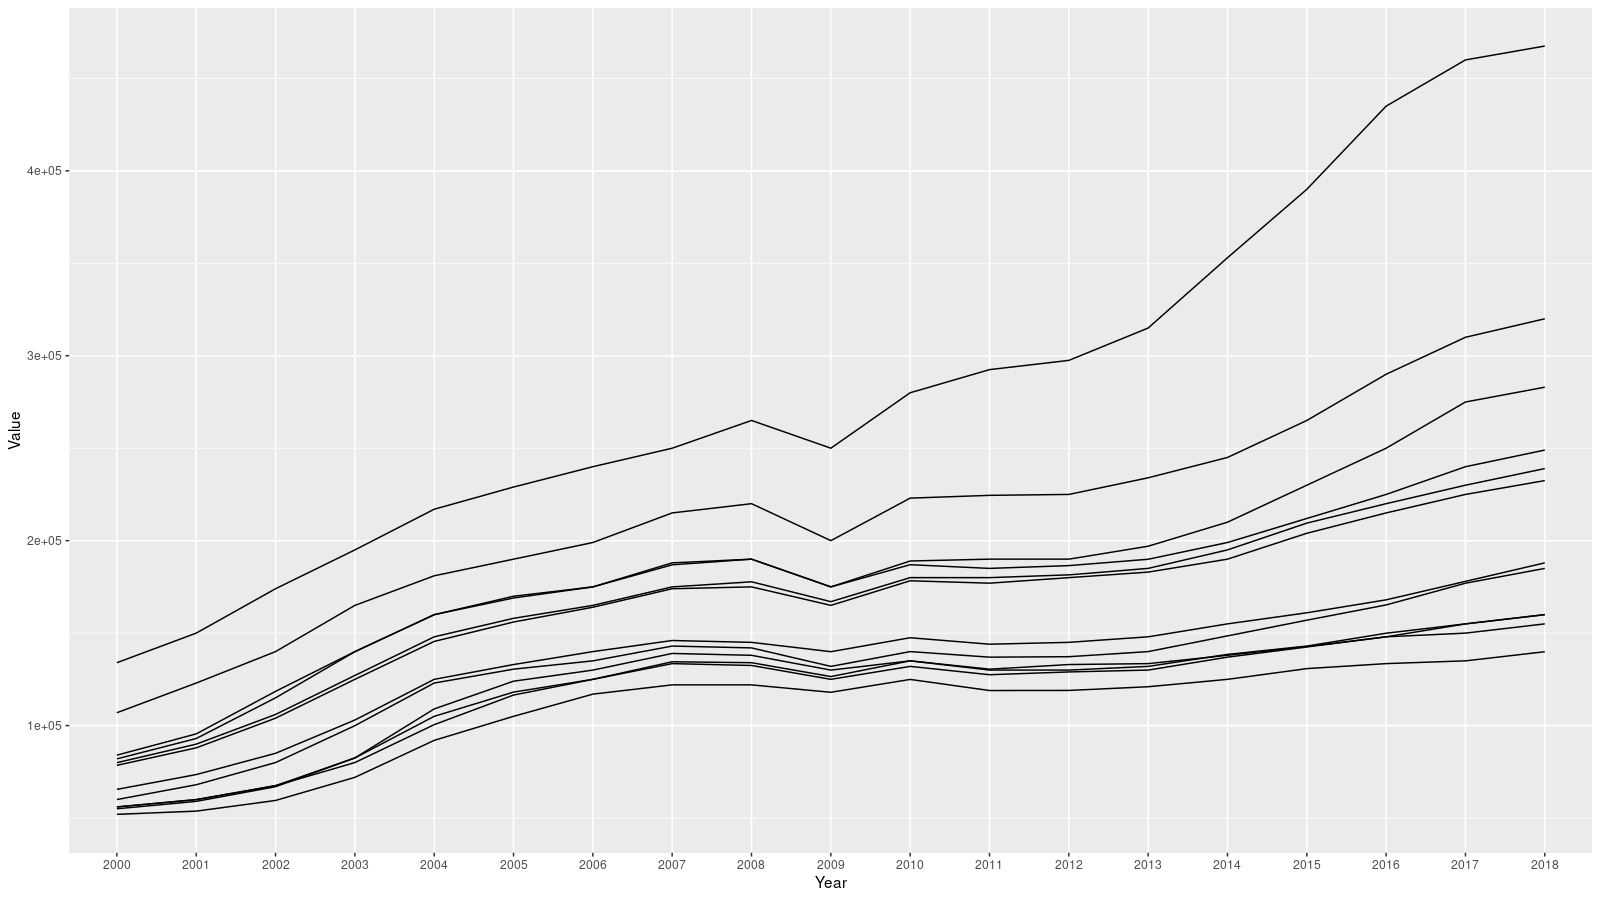
\includegraphics[width=8.5cm]{Q1Geom_line_no_colour}}
  %  \vspace{2.0cm}
    \centerline{Q1 Line Graph No Colour}\medskip
  \end{minipage}
\end{figure}

\begin{figure}[H]
  \begin{minipage}[b]{1.0\linewidth}
    \centering
    \centerline{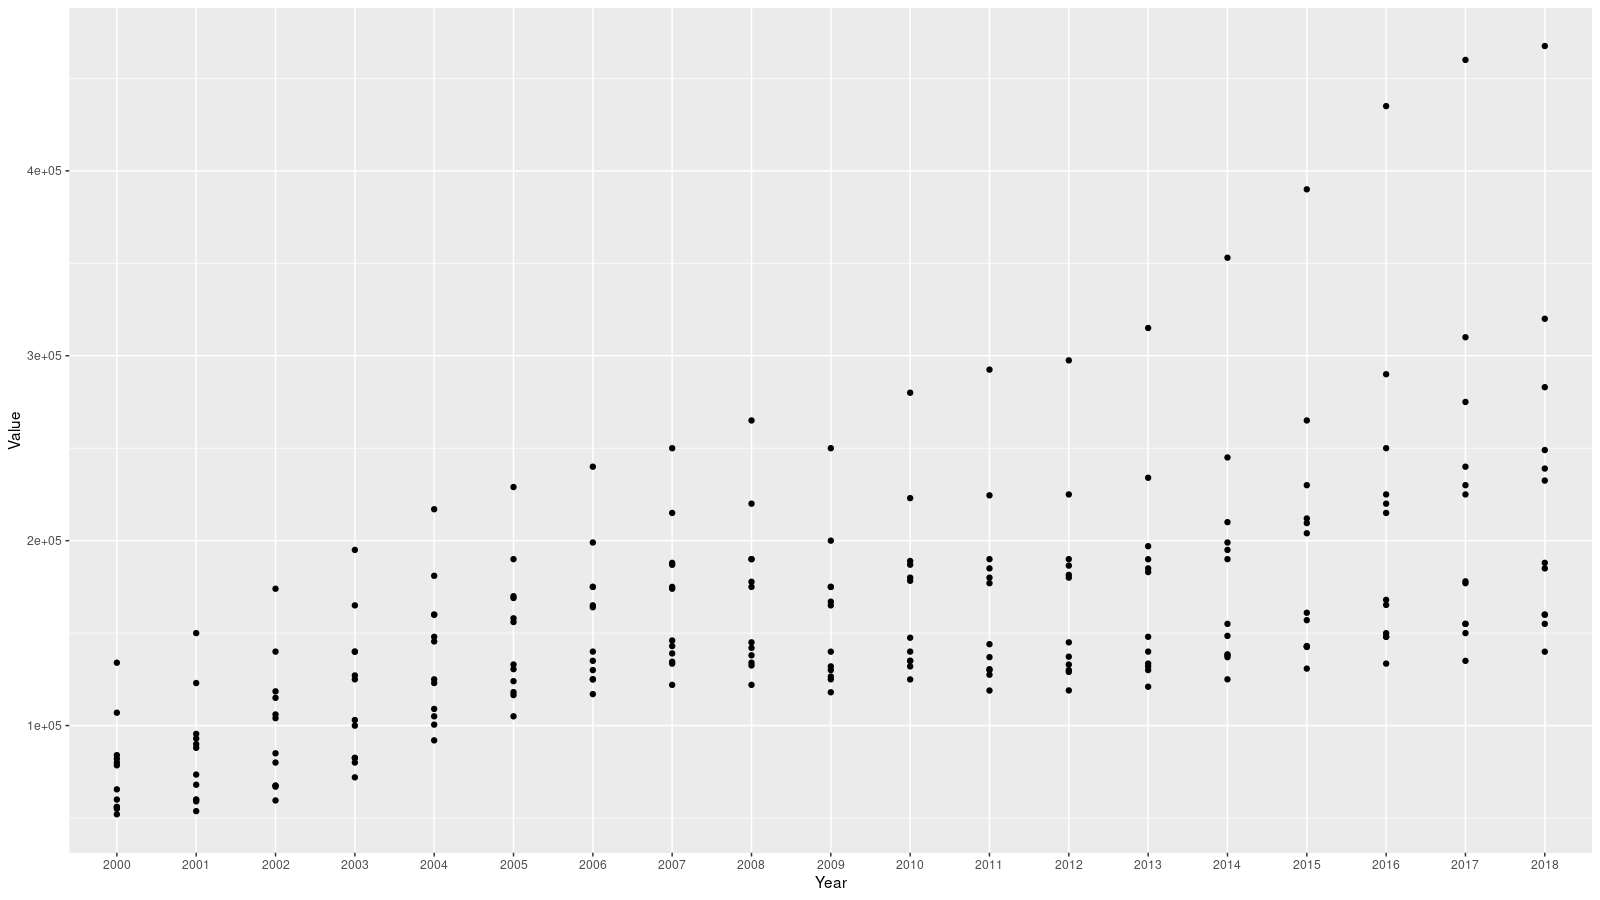
\includegraphics[width=8.5cm]{Q1Geom_point_no_colour}}
  %  \vspace{2.0cm}
    \centerline{Q1 Dot Plot No Colour}\medskip
  \end{minipage}
\end{figure}

\begin{figure}[H]
  \begin{minipage}[b]{1.0\linewidth}
    \centering
    \centerline{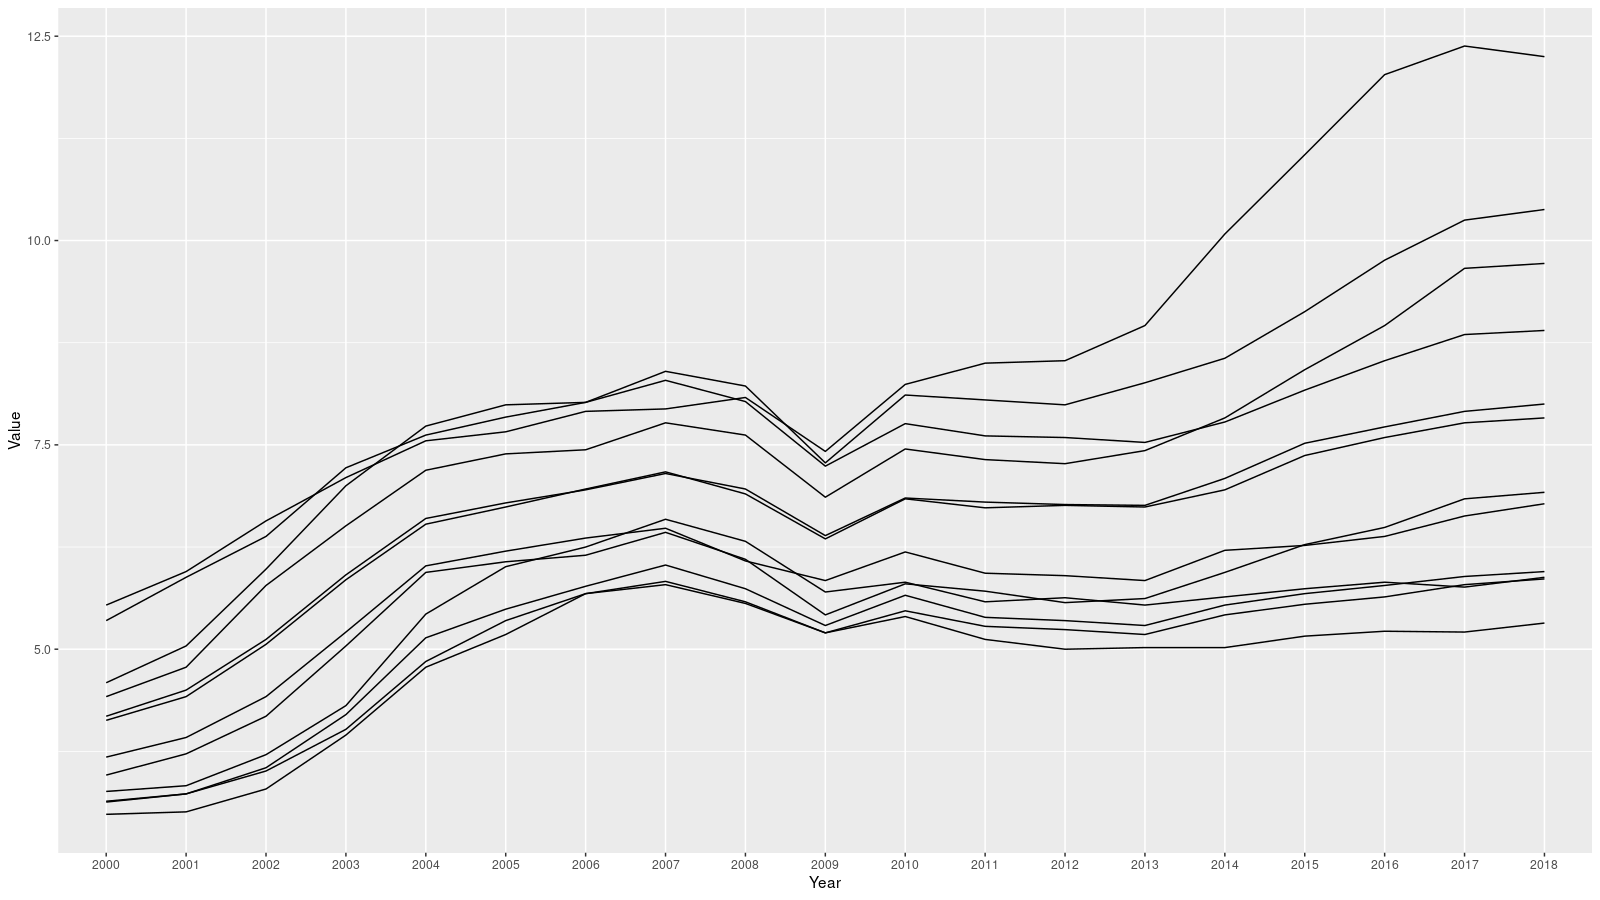
\includegraphics[width=8.5cm]{Q2Geom_line_no_colour}}
  %  \vspace{2.0cm}
    \centerline{Q2 Line Graph No Colour}\medskip
  \end{minipage}
\end{figure}

\begin{figure}[H]
  \begin{minipage}[b]{1.0\linewidth}
    \centering
    \centerline{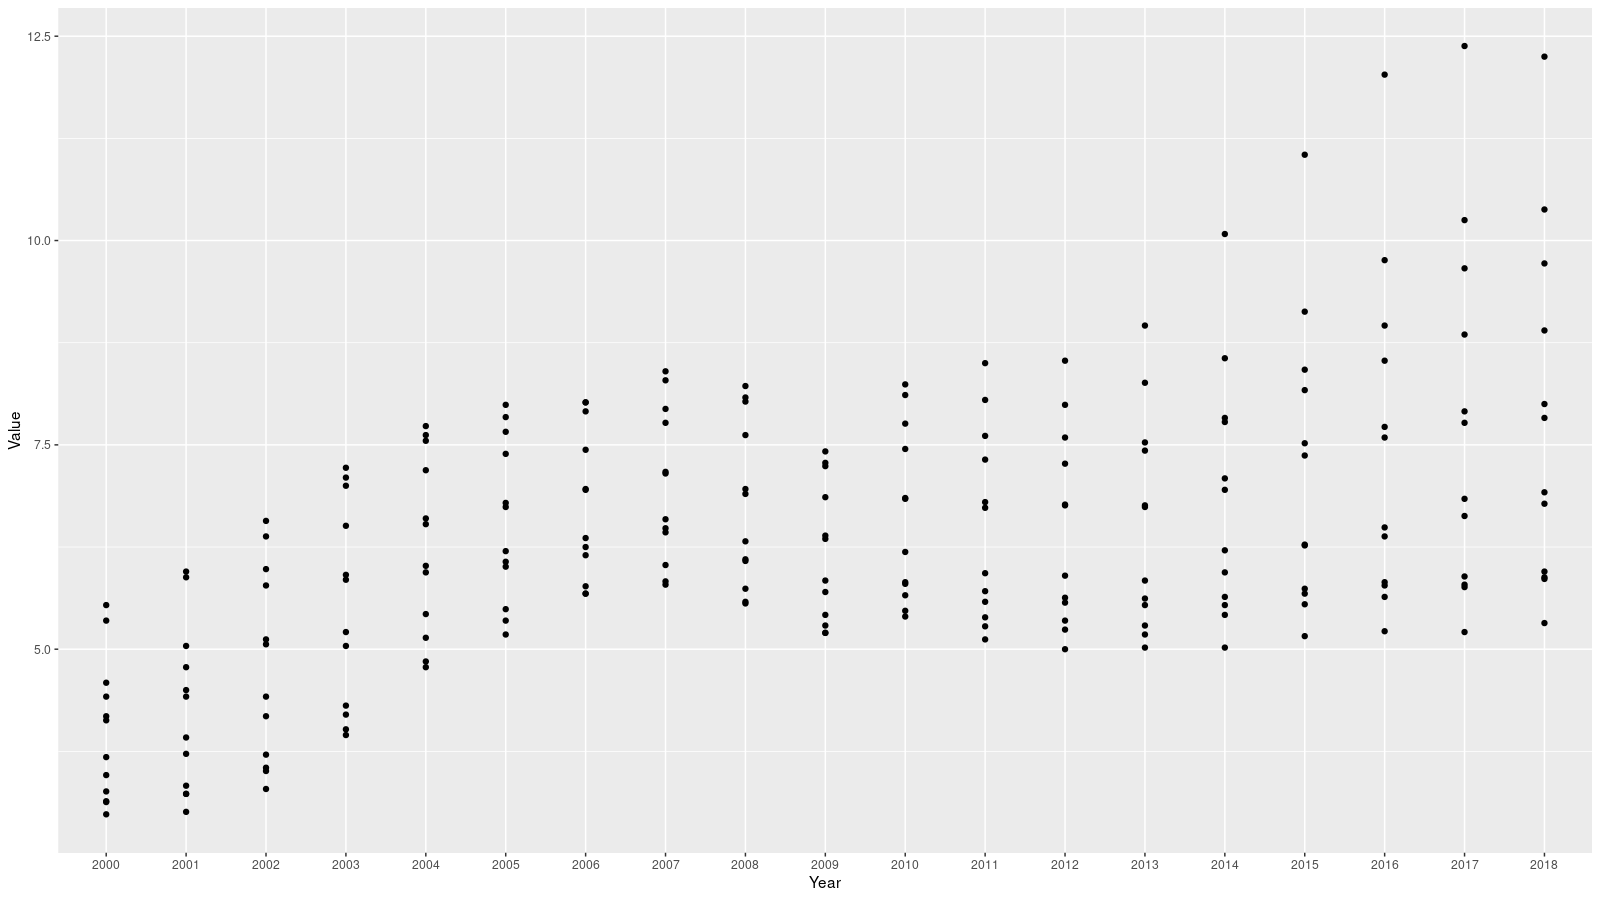
\includegraphics[width=8.5cm]{Q2Geom_point_no_colour}}
  %  \vspace{2.0cm}
    \centerline{Q2 Dot Plot No Colour}\medskip
  \end{minipage}
\end{figure}

\subsection{Appendix 2}
\begin{figure}[H]
  \begin{minipage}[b]{1.0\linewidth}
    \centering
    \centerline{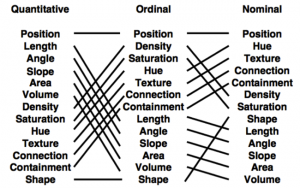
\includegraphics[width=8.5cm]{mackinlayRankings}}
  %  \vspace{2.0cm}
    \centerline{Mackinlay's Effectiveness Rankings}\medskip
  \end{minipage}
\end{figure}



\end{document}
